\section{Video Similarity Application}
\label{sec:Video Similarity Application}
GhostPeerShare uses the CKKS \cite{Cheon2017-CKKS} fully homomorphic scheme for all encryption arithmetic. Specifically, this scheme uses three security parameters: 1) Polynomial Modulus Degree, 2) Encoder Scalar, and 3) Sizes of the Coefficient Modulus Chain (qSizes). The Polynomial Modulus Degree configures the size of the ciphertext and the number of slots available for encoding data. Next, CKKS encodes real numbers into polynomials, and the encoder scalar is used to scale real numbers by a significant factor to preserve precision. Finally, the Sizes (in bits) in the Coefficient Modulus Chain contribute to the noise budget. The modified ciphertext cannot be decrypted if too much noise is introduced. By default, GhostPeerShare selects the Polynomial Modulus Degree of 4096, Encoder Scalar of $2^{40}$, and qSizes of [60, 40, 40, 60].

In order to detect similarities between the two videos, we represent each video as a probability distribution of byte size changes between one-second segments, shown in Figure \ref{fig:preprocess-data-flow}. To transform raw video into comparable probability distributions, we count the number of bytes in each frame, calculate the sum of frame lengths in each segment, and then normalize the array of segments between zero and one, known as a Probability Distribution Form (PDF), ensuring that the distributions for both videos have the same scale and can be directly compared. This re-implementation of Proof of Presence Share \cite{Lagesse2021-PopShare} provides strong privacy guarantees, as if the encryption is broken, the raw byte data cannot be reconstructed from the normalized byte array due to the loss of information during the aggregation and normalization process. Alternative approaches include a motion estimation approach with the Lucas-Kanade method \cite{Lucas1981-uy} supported by OpenCV, which could provide more detailed information about video content. However, for this study, it is crucial to compare our approach to the established baseline metrics, and new methods would hinder this comparison.

\begin{figure}[t]
    \centering
    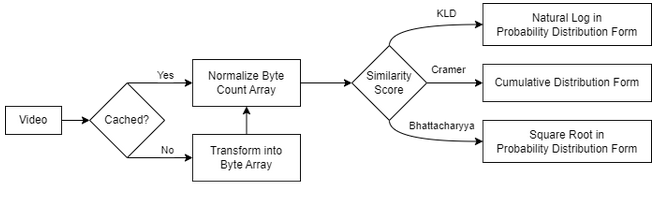
\includegraphics[width=\textwidth]{4 Design/4.3 Preprocess Data Flow.png}
    \caption{Pre-process Data Flow}
    \label{fig:preprocess-data-flow}
\end{figure}

To compute multiple similarity scores using homomorphic encryption, separate byte arrays are encrypted for each score. The recipient can perform computations with plaintext decimal values against the corresponding encrypted element in the array. This approach leverages the unique ability of fully homomorphic encryption and was borrowed from Pop-Share, as this approach is much faster than comparing ciphertext against ciphertext. 

For Kullback-Leibler Divergence (KLD), we share the PDF and its natural log. For each encrypted double in the PDF, we subtract the natural log of the plaintext element and multiply the difference. The product remains encrypted and is returned to the originator, where it can be decrypted. The summation is the similarity score.

For Bhattacharyya Coefficient (BC), we share the square root of the PDF. For each encrypted double, we multiply the ciphertext by the square root of the plaintext element. The product remains encrypted and is returned to the originator, where it can be decrypted. The summation is the similarity score.

For Cramer Distance (CD), we share the Cumulative Distribution Form (CDF) derived from PDF. The CDF is the cumulative sum of all of the elements in the PDF, such that the last value of CDF is equal to 1. For each encrypted double, we square the difference of the plaintext element. The product remains encrypted and returned to the originator, where it can be decrypted, and the square root of the summation is the similarity score.

\begin{figure}[t]
    \centering
    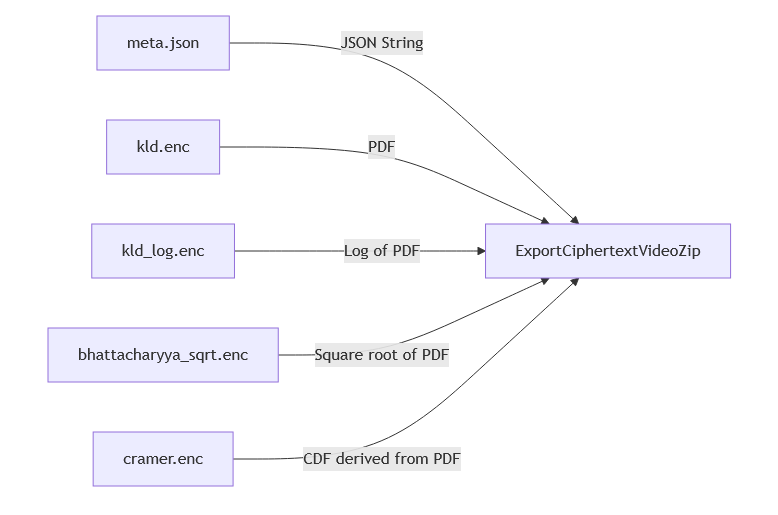
\includegraphics[width=\textwidth]{4 Design/4.3 Archive.png}
    \caption{Serialized Ciphertext Archive}
    \label{fig:ciphertext-archive-contents}
\end{figure}

In order to share the encrypted byte-count arrays, GhostPeerShare packages all ciphertext objects into an archive, the contents illustrated in Figure \ref{fig:ciphertext-archive-contents}. The \textit{meta.json} files contain all computed metadata about the video file, including the timestamp, frames per second, and duration. For a one-minute video, each encrypted archive, files ending with \textit{.enc}, contains 60 binary files, each representing a one-second segment. Each binary file contains an encrypted floating-point number. This structure is useful for cases where the two videos are different lengths, simplifying the trimming process. The \textit{kld.enc} and \textit{kld\_log.enc} are the binary archives containing the encrypted parameters to compute the KLD distance measure scores. The \textit{kld.enc} binary archive contains the encrypted PDF. The \textit{kld\_log.enc} binary archive contains the encrypted logarithm of PDF. The \textit{bhattacharyya\_sqrt.enc} binary archive contains the encrypted square root of PDF. The \textit{cramer.enc} binary archive contains the encrypted CDF. The serialized archive, \textit{ExportCiphertextVideoZip} contains all binary archives and metadata files. In total, the serialized archive averages around 40 MB on Linux and Android for 1 minute of video.

\begin{figure}[t]
    \centering
    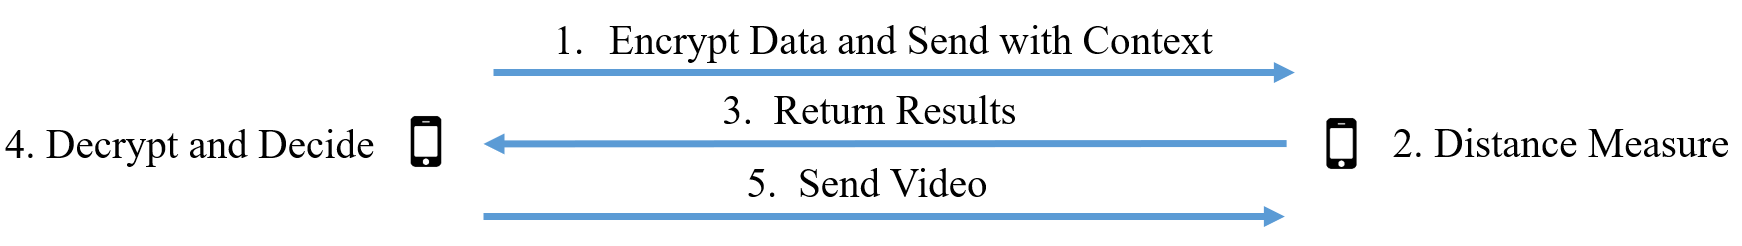
\includegraphics[width=\textwidth]{4 Design/4.3 Peer-to-Peer.png}
    \caption{Peer-to-peer Data Flow}
    \label{fig:peer-to-peer-data-flow}
\end{figure}

To facilitate a peer-to-peer exchange of files shown in Figure \ref{fig:peer-to-peer-data-flow}, GhostPeerShare supports QuickShare \cite{samsung_quick_2020} for Android devices. QuickShare \cite{samsung_quick_2020} was developed by Samsung as a file-sharing utility application for nearby wireless devices. It leverages Bluetooth to discover nearby wireless devices and optionally uses WiFi to transfer large files between two nodes. QuickShare is accessible through a Flutter plugin that enables users to share data using their device’s native sharing capabilities. This allows each node to asynchronously send and receive files, leveraging a built-in Android feature rather than embedding similar functionality within the Flutter application.

